\documentclass[conference]{IEEEtran}
\IEEEoverridecommandlockouts \overrideIEEEmargins 
%\pagestyle{plain}
\usepackage{fullpage}
\usepackage[ruled,vlined,linesnumbered]{algorithm2e}
\usepackage{mathrsfs}
\usepackage{graphicx}
\usepackage{amsfonts}
\usepackage{amsmath}
\usepackage{amssymb}
\usepackage{array}
\usepackage{flafter}
%\usepackage{cite}
\usepackage{subfigure}
\usepackage{verbatim}
%\usepackage{bbm}
\usepackage[usenames]{color}
\usepackage[svgnames]{xcolor}
\usepackage{psfrag}
\usepackage{umoline}
\usepackage{hyperref}
%\usepackage{appendix} %[2009/09/02 v1.2b extra appendix facilities]
\let\proof\relax
\let\endproof\relax
\usepackage{amsthm}	% This is needed for \newtheorem and proof environment.
%\usepackage{natbib} % for citing the papers with auther-year format in parantheses.

\providecommand{\citet}[1]{\citeauthor{#1}\,[\citeyear{#1}]}
\providecommand{\citep}[1]{\cite{#1}}

\newtheorem{thm}{Theorem}
\newtheorem{Def}{Definition}
\newtheorem{Problem}{Problem}
\newtheorem{Lem}{Lemma}
\newtheorem{Cor}{Corollary}
\newtheorem{assumption}{Assumption}
\newtheorem{proposition}{Proposition}
\newtheorem{definition}{Definition}
\newtheorem{property}{Property}
\newtheorem{Remark}{Remark}
\newtheorem{exmp}{Example}[section]
%\newenvironment{proof}[1][Proof]{\begin{trivlist}
%\item[\hskip \labelsep {\bfseries #1}]}{\end{trivlist}}

\newcommand{\TypeOfDoc}{IJRR} % This either can be TR or Conf or IJRR
\newcommand{\FinalFlag}{No} % This either can be No or Accepted

\graphicspath{{./figs/}}

\allowdisplaybreaks[1]

%\newcommand{\kXX}[1]{\color{blue} XX #1 XX \color{black}}
%\newcommand{\AXX}[1]{\color{orange} XX #1 XX \color{black}}
\newcommand{\aXX}[1]{\color{purple} #1 \color{black}}


%*********************************************************%
%	 	Shortcuts				  %
%*********************************************************%
\newcommand\mI{\mathbf{I}}
\newcommand\mJ{\mathbf{J}}
\newcommand\mIJ{\left(\mI-\mJ\right)}
\newcommand\mIJkIJ{\left(\mIJ\kro\mIJ\right)}
\newcommand\mM{\mathbf{M}}
\newcommand\mK{\mathbf{K}}
\newcommand\mA{\mathbf{A}}
\newcommand\mB{\mathbf{B}}
\newcommand\mD{\mathbf{D}}
\newcommand\mR{\mathbf{R}}
\newcommand\mS{\mathbf{S}}
\newcommand\mQ{\mathbf{Q}}
\newcommand\mE{\mathbf{E}}
\newcommand\mL{\mathbf{L}}
\newcommand\mP{\mathbf{P}}
\newcommand\mH{\mathbf{H}}
\newcommand\mC{\mathbf{C}}
\newcommand\IDm{(\mI+\mD)^{-1}}
\newcommand\UL{{U^L}}
\newcommand\mk{m_{\mathcal{K}}}
\newcommand\pk{p_{\mathcal{K}}}

\newcommand\vOne{\mathbf{1}}
\newcommand\vx{\mathbf{x}}
\newcommand\vv{\mathbf{v}}
\newcommand\vs{\mathbf{s}}
\newcommand\vw{\mathbf{w}}
\newcommand\vu{\mathbf{u}}

\newcommand\kro{\otimes}
\newcommand\Tr{\mathrm{Trace}}
\newcommand\LRN{\left|\!\left|\!\left|}
\newcommand\RRN{\right|\!\right|\!\right|}

\newcommand\E{\mathbb{E}}
\newcommand\Prob{\mathbb{P}}
\newcommand{\e}{{\mathrm e}}
\newcommand\T{^{\mathrm T}}

\newcommand\cvd{\xrightarrow[]{\ \mathcal{D}\ }}
\newcommand\cvp{\xrightarrow[]{\ \mathbb{P}\ }}
\newcommand\cvas{\xrightarrow[]{\ \mathrm{a.s.}\ }}
\newcommand\cvL{\xrightarrow[]{\ L^1\ }}
\newcommand\cvLL{\xrightarrow[]{\ L^2\ }}
\newcommand\cvLp{\xrightarrow[]{\ L^p\ }}
\newcommand\smallo{{{\scriptstyle\mathcal{O}}}}

\newcommand\ie{{\it i.e. }}
\newcommand\etal{{\it et al. }}

\usepackage{amsthm}
\newtheorem{theorem}{Theorem}[section]
\newtheorem{lemma}[theorem]{Lemma}
\usepackage{amssymb}
\usepackage{nomencl}
\usepackage{balance}
\usepackage{todonotes}
\usepackage[author={Max Schlepzig}]{pdfcomment}

\DeclareFontFamily{OT1}{pzc}{}
\DeclareFontShape{OT1}{pzc}{m}{it}{<-> s * [1.10] pzcmi7t}{}
\DeclareMathAlphabet{\mathpzc}{OT1}{pzc}{m}{it}
\DeclareMathOperator*{\argmin}{argmin}  
\makenomenclature
\usepackage{xifthen}
\usepackage{hyperref}
\usepackage{xparse}
%\newcommand{\vect}{\bf}
\newcommand{\vect}[1]{{\mathbf{#1}}}
\newcommand{\matr}{\bf}
\newtheorem{prop}{Proposition}
\theoremstyle{remark}
\newtheorem{remark}{Remark}
\usepackage{pgfplots} 
\newlength\figureheight 
\newlength\figurewidth
\pgfplotsset{compat=newest} 
\pgfplotsset{plot coordinates/math parser=false} 
%\renewcommand{\footnotesize}{\footnotesize}
\renewcommand{\footnotesize}{\fontsize{7.5pt}{9pt}\selectfont}
%\usepackage{enumitem}

\newcommand{\tl}[1]{{\color{orange} - Fix Language: #1 - \ }}  % Typo or 
%Language
\newcommand{\axx}[1]{{\color{blue} AT: #1  \ }}  % AmirHossein's comments
\newcommand{\dxx}[1]{{\color{green} DS: #1  \ }}  % Dylan's comments
\newcommand{\rxx}[1]{{\color{orange} RO: #1  \ }}  % Reza's comments
\newcommand{\sxx}[1]{{\color{red} SC: #1  \ }}  % Suman's comments
\newcommand{\nxx}[1]{#1}  % approved

\newcommand{\bxx}[1]{{\color{blue} - T: #1 - \ }}  % AmirHossein's comments
\newcommand{\XX}[3][2]{\mathbf{X}_{\tiny #2}^{\tiny #3}}
\newcommand{\pr}{\textrm{p}}
\newcommand{\pp}[3][2]{\pr(x #2 | #3)}

%\newcommand{\bIn}{\boldsymbol{I}_{\boldsymbol{n}}}
%\newcommand{\bIa}{\boldsymbol{I}_{\boldsymbol{a}}}
%\newcommand{\bIk}{\boldsymbol{I}_{\boldsymbol{k}}}
%\newcommand{\bIkk}{\boldsymbol{I}_{\boldsymbol{k-1}}}

\newcommand{\bIn}{\boldsymbol{I}_{{n}}}
\newcommand{\bIa}{\boldsymbol{I}_{{a}}}
\newcommand{\bIk}{\boldsymbol{I}_{{k}}}
\newcommand{\bIkk}{\boldsymbol{I}_{{k-1}}}
\newcommand{\bIs}[1]{\boldsymbol{I}_{#1}}  % Suman's comments
\newcommand{\xx}[3][2]{\mathbf{x}_{ #2}^{ #3}}
\newcommand{\zz}[3][2]{\mathbf{z}_{ #2}^{ #3}}
\newcommand{\ZZ}[3][2]{\mathbf{Z}_{ #2}^{ #3}}
\newcommand{\ZZh}[3][2]{\mathbf{\hat{z}}_{ #2}^{ #3}}
%\newcommand{\yy}[3][2]{\mathpzc{y}_{\tiny #2}^{\tiny #3}}
%\newcommand{\YY}[3][2]{\mathpzc{Y}_{\tiny #2}^{\tiny #3}}

\newcommand{\yy}[3][2]{\psi^{\tiny #3}({\tiny #2})}
\newcommand{\YY}[3][2]{\phi^{\tiny #3}({\tiny #2})}
\newcommand{\suf}[1]{\textsc{\tiny #1}}  % Suman's comments

\newcommand{\ii}[3][2]{\overline{\delta \mathpzc{i}}_{\tiny {#2}}^{\tiny {#3}}}
\newcommand{\II}[3][2]{\overline{\delta \mathpzc{I}}_{\tiny {#2}}^{\tiny {#3}}}
\newcommand{\psx}{p_*(\vect{x})}
\newcommand{\pcfx}{p_{\textsc{\tiny CF}}(\vect{x})}
\newcommand{\phybx}{p_{\textsc{\tiny HYB}}(\vect{x})}
\newcommand{\pixz}{\tilde{p}^i(\xx[]{k}{}\vert \vect{Z}_{k})}
\newcommand{\pixzm}{\tilde{p}^i(\xx[]{k}{}\vert \vect{Z}_{k-1})}
\newcommand{\pzix}{\tilde{p}^i( \vect{z}_{k} \vert \xx[]{k}{})}
\newcommand{ \pcf}{\frac{1}{\eta_{\textsuperscript{CF}}}\prod_{i=1}^{N} \pr(\vect{z}_{k}^i | \xx[]{k}{})^{\omega_i} \prod_{i=1}^{N} \tilde{p}^i(\vect{x}_{k} | \vect{Z}_{k-1})^{\omega_i}}
\newcommand{ \phyb}{\frac{1}{\eta_{\textsc{\tiny HYB}}}\prod_{i=1}^{N} \pr(\vect{z}_{k}^i | \xx[]{k}{}) \prod_{i=1}^{N} \tilde{p}^i(\vect{x}_{k} | \vect{Z}_{k-1})^{\bar{\omega}_i} }
\newcommand{ \pstar}{\frac{1}{\eta_*} \{ \prod_{i=1}^{N} \pr(\vect{z}_{k}^i | \xx[]{k}{}) \} \pr(\xx[]{k}{}|\vect{Z}_{k-1})}
 
\newcommand{ \npcf}{\prod_{i=1}^{N} \pr(\vect{z}_{k}^i | \xx[]{k}{})^{\omega_i} \prod_{i=1}^{N} \tilde{p}^i(\vect{x}_{k} | \vect{Z}_{k-1})^{\omega_i}}
\newcommand{ \nphyb}{\prod_{i=1}^{N} \pr(\vect{z}_{k}^i | \xx[]{k}{}) \prod_{i=1}^{N} \tilde{p}^i(\vect{x}_{k} | \vect{Z}_{k-1})^{\bar{\omega}_i} }
\newcommand{ \npstar}{ \{ \prod_{i=1}^{N} \pr(\vect{z}_{k}^i | \xx[]{k}{}) \} \pr(\xx[]{k}{}|\vect{Z}_{k-1})}
 
\DeclareDocumentCommand{\ais}{m m m  }{{#1}_{#2}^{#3}}
\DeclareDocumentCommand{\bis}{m m m  }{{#1}_{{\tiny #2}}^{{\tiny #3}}}
\DeclareDocumentCommand{\cis}{m m m  }{{#1}_{{\tiny #2}}^{{\tiny {#3}}}}
\newcommand{\ti}[1]{\textsc{\tiny #1}}
\newcommand{\lrp}[1]{\left( #1 \right) }

\allowdisplaybreaks[1]

\usepackage{algpseudocode}% http://ctan.org/pkg/algorithmicx
\usepackage{microtype}
\usepackage{lipsum}

\title{\LARGE \bf Efficient Distributed State Estimation of\\ Hidden Markov Models over Unreliable
	Networks}
\author {Amirhossein Tamjidi$^{1}$, Reza Oftadeh$^{2}$, Suman Chakravorty$^{1}$, Dylan Shell$^{2}$
\thanks{$^{1}$Department of Aerospace Engineering, Texas A\&M University}
\thanks{$^{2}$Department of Computer Science \& Engineering, Texas A\&M University}
\thanks{Corresponding author email: ahtamjidi@tamu.edu}}

\begin{document}
	
	\maketitle
\begin{abstract}
This paper presents a new recursive Hybrid consensus filter for 
distributed state estimation on a Hidden Markov Model (HMM), which is 
well-suited to multi-robot applications and settings. The proposed algorithm is 
\textit{scalable}, \textit{robust to network failure} and capable of handling 
\textit{non-Gaussian} transition and observation models and, therefore, it is 
general. No global knowledge of the communication network is assumed. Iterative 
Conservative Fusion (ICF) is used to reach consensus over potentially 
correlated priors, while consensus over likelihoods is handled using weights 
based on a Metropolis Hastings Markov Chain (MHMC). The proposed method is 
evaluated in a multi-agent tracking problem and a high dimensional HMM and it 
is shown that  its performance surpasses the competing algorithms. 
\end{abstract}

\section{Introduction}
Estimation within robotic-sensor networks has many applications and, thus, has been 
extensively studied in recent years 
\cite{durrant2001data,campbell2016distributed,boem2015decentralized}. In a 
 mobile sensor network, robots carry sensors that make noisy observations of the 
state of an underlying system of interest. The estimation is considered 
centralized if all the nodes send their raw observations to a central node who 
then calculates an estimate based on the collective information 
\cite{ahmed201522}. This is not always possible owing to link failures as well as 
bandwidth and energy constraints \cite{Zhang_ttradeof1}. One viable alternative 
is Distributed State Estimation (DSE).

In DSE, the processor on each node (or robot) fuses local information with the incoming information from neighbors and redistributes the fused result on the network. The objective is to design both a protocol for message passing between nodes and local fusion rules so that the nodes reach a consensus over their collective information. Although the DSE algorithms are not guaranteed to match the performance of the centralized estimator all the time, their scalability, modularity and, robustness to network failure motivates the ongoing research. These features are important for the envisioned robotic applications of such algorithms, such as multi-agent localization \cite{5509143} and cooperative target tracking \cite{whitacre2013cooperative}. 

DSE algorithms can be categorized on the basis of assumptions they make. Any 
DSE method makes assumptions about one or more of the following aspects: the 
state (static \cite{xiao2005scheme} or dynamic \cite{5509143}), state 
transition model (linear \cite{olfati2005distributed} or non-linear 
\cite{battistelli2014parallel,rao2003constrained,boem2013distributed,hu2014state}),
 type of noise (Gaussian 
\cite{xiao2005scheme,olfati2005distributed} or non-Gaussian 
\cite{hlinka2013distributed}), topology of the network (constant or changing 
\cite{tamjidi2016unifying,xiao2005scheme}), connectivity of the network (always 
\cite{battistelli2014parallel} or intermittent connection 
\cite{tamjidi2016unifying,xiao2005scheme}), agents' knowledge about the network 
topology (global or local 
\cite{tamjidi2016unifying,xiao2005scheme,battistelli2014parallel}) and finally 
the treatment of  mutual information between local estimate (exact solution 
through bookkeeping \cite{durrant2001data} or conservative  solutions that 
avoid double counting \cite{wang_distr_CI,hu2012diffusion}).

The research on DSE for linear systems with Gaussian noise is extensive (see 
\cite{olfati2005distributed,cattivelli2010diffusion} for reviews). For 
nonlinear systems with Gausssian noise, the distributed versions of Extended 
Kalman Filters (EKF), Extended Information Filters (EIF) and Unscented Kalman 
Filter (UKF) have been proposed  
\cite{battistelli2016stability,dist_inf_filter_2009,battistelli2014parallel}, 
respectively. For nonlinear systems with non-Gaussian noise, different flavors 
of Distributed Particle Filter (DPF) methods were proposed by Mao and Yang
\cite{lin_dist_part_filter_2014}. 

For dynamic state systems within time-varying networks, the connectivity constraint is a determining factor for 
choosing the proper DSE method. If the network remains connected, DSE methods 
can maintain equality of each node's priors and then perform consensus on likelihoods only 
\cite{hlinka2012likelihood,li2012distributed}. We refer to this approach as 
Consensus on Likelihoods (CL). The advantage of CL is that given enough time to 
reach consensus, it can match the centralized estimator's performance. However, 
if the network becomes disconnected, priors become different and CL methods 
fail. In such scenarios, the prevailing  approach is to perform Iterative 
Conservative Fusion (ICF) on node posteriors 
\cite{battistelli2014kullback,wang_distr_CI,hu2012diffusion}. ICF methods have a conservative fusion rule that 
avoids double counting at the expense of down weighting the uncorrelated 
information. Consequently, they are inherently sub-optimal.

Researchers recently began combining ICF and CL 
methods to benefit from their complementary features 
\cite{battistelli2016stability,battistelli2014parallel,tamjidi2016unifying}: CL 
can reach consensus over uncorrelated new information, while ICF can handle  
correlated prior information. 
%It is worth noting that the logic behind the Hybrid method is intuitive once explained yet, it has long been neglected. 
In this paper we extend our previous method \cite{tamjidi2016unifying} to 
general finite-state systems with non-Gaussian noise. We propose a 
\emph{Hybrid} method that is a synergistic combination of \axx{CL} and ICF.
The contributions of the 
paper are:
\begin{itemize}
\item The new Hybrid method shows unmistakable superiority over ICF in applications with large number of agents and time-varying networks that face intermittent disconnection. 
\item The method handles non-Gaussian noise models 
which is particularly 
useful for collaborative tracking and localization applications.
\end{itemize}

Hidden Markov Models (HMMs) are adopted as the general means for describing the system whose state is being estimated.  In Section~\ref{subsec:assump_not}, the notation used in this paper is explained as well 
as assumptions, along with the system model. Section~\ref{subsec:Preliminaries} discusses 
some preliminaries on distributed state estimation, paving the way for the new  
method. Our proposed method is presented in Section \ref{subsec:Method} and finally, we evaluate its performance in Section 
\ref{sec:experiments}.  

\section{Notation and Modeling} \label{subsec:assump_not}
\subsubsection*{The Network Topology} 
Assume that we have $n$ homogeneous agents associated with the nodes of a 
graph. These agents can communicate with each other under a time-varying 
undirected network topology $ G_{k} = \langle \mathcal{V},\mathcal{E}_k\rangle 
$ where $\mathcal{V}$ and $\mathcal{E}_k$ are the set of graph nodes and edges 
at step $k$ respectively. The node corresponding to the $i^\text{th}$ agent is 
denoted by $v_i$. If $(v_i,v_j)\in \mathcal{E}_k$, it means that agents $i$ and 
$j$ can communicate directly at step $k$.  The set $\overline{\mathcal{N}}_i$ 
represent 
neighbors of node ${v}_i$ that are connected by an edge to $v_i$. The set 
$\mathcal{N}_i=\overline{\mathcal{N}}_i\cup \{v_i\}$ will also be used in some 
of the equations. The set $\textsc{CC}_k^i$ represents the set of agents 
that are \textit{path-connected} to agent $i$ at step $k$. For an arbitrary set 
with 
$s\in \mathbb{N} $ members $\mathbf{b}=\{b_{i_1},\cdots,b_{i_s}\}$, 
the index set $\boldsymbol{I}_{b}=\{i_1,\cdots,i_{s}\}$ 
contains the indices of $\mathbf{b}$'s members. We use the abbreviated form  $ 
\bIn = 
\{1,2,\cdots,n\},$ and $\bIk = \{1,2,\cdots,k\}$ to index the agents and time 
steps, respectively.

\subsubsection*{The Model} Consider a finite state HMM with the following specification:
\begin{itemize}
	\item The HMM has $n_s$ possible states $\mathcal{X} = \{S_1,\cdots,S_{n_s}\} $ and also, there are $n_z$ possible observation symbols $\mathcal{Z} = \{O_1,\cdots,O_{n_z}\}$.
	\item The random variables $\vect{X}_k \in \mathcal{X} $ and $ \vect{Z}_k^i \in \mathcal{Z} $ represent the state and observation made by agent $i$ at step $ k $, respectively. The realizations of those random variables at step $k$ are denoted as $\vect{x}_k$ and $\vect{z}_k^i$.    
	\item The transition model is a $n_s\times n_s$ matrix denoted as $\mathcal{P}_{k \vert k-1}\triangleq \pr(\vect{X}_{k} | \XX[]{k-1}{})$. All the agents possess this model.
	\item \axx{Each agent has} an observation model, which is a $n_s\times n_z$ 
	matrix denoted as $\pr(\vect{Z}_{k}^{i} | \vect{X}_{k}), i\in\bIn$. The 
	observation models of different agents can differ.
	\item The prior, prediction, and posterior probabilities are $1\times n_s$ random vectors
	\begin{align}
		\pi_{k-1}&\triangleq \pr\left(\XX[]{k-1}{}|\{\zz{k}{i}\}^{i\in\bIn}_{k\in\bIkk}\right),\nonumber\\
		\tilde{\pi}_{k}&\triangleq \pr\left(\XX[]{k}{}|\{\zz{k}{i}\}^{i\in\bIn}_{k\in\bIkk},\XX[]{k-1}{}\right),\nonumber\\
		\pi_{k}&\triangleq \pr\left(\XX[]{k}{}|\{\zz{k}{i}\}^{i\in\bIn}_{k\in\bIk}\right),\nonumber
	\end{align}
	respectively.
\end{itemize}
The above HMM is well-defined for many distributed estimation applications including ones with dynamic state and time varying observation models. For example, the following transition and observation models can be represented in the above form:
\begin{align}
\XX[]{k+1}{} &= f(\XX[]{k+1}{},\ais{\vect{w}}{k}{})\quad \ais{\vect{w}}{k}{} \sim \pr(\ais{\vect{W}}{k}{}), \\
\ZZ{k+1}{i} &= h^i(\XX[]{k+1}{},\ais{\vect{v}}{k}{})\quad \ais{\vect{v}}{k}{} \sim \pr(\ais{\vect{V}}{k}{}), 
\end{align}
in which, $\ais{\vect{W}}{k}{}$ and $\ais{\vect{V}}{k}{}$ are random variables representing dynamics and observation noise. We further assume that each agent has a processor and a sensor on-board. Sensors make observations every $\Delta t$ seconds and the processors and the network can handle calculations based on message passing among agents every $\delta t$ seconds. We assume that $\delta t \ll \Delta t$. We also assume that the agents exchange their information over the communication channel which is free of both delay and error. Note that the above specification for the HMM and the model may easily be extended to include control inputs but they are omitted as they are not the focus this paper. 

Henceforward, $\{\ZZ{k}{i}\}^{i\in\bIn}_{k\in\bIk}$ is the indexed family of all the 
observations made by all the agents up to step $k$. Moreover, for each agent 
$i$, the variable $\vect{R}_{k}^{ij}, j \in \overline{\mathcal{N}}_i $ denotes 
the information that node $i$ receives from node $j$, its neighbor at time 
$k$. The set $\vect{R}_{k}^i$ contains all the information that node $i$ has 
received from its neighbors up to step $k$ and $\vect{I}_{k}^i = \vect{R}_{k}^i 
\cup \vect{Z}_{k}^i$ represents all the information content that is available 
to agent $i$ at time $k$. (In 
general, in this paper, the information in the 
variable that bears the superscript $i$ is a version local to the $i^\text{th}$ 
agent. Moreover, symbol $\eta$ with or without any sub/superscript is a 
normalizing constant.)
\nomenclature{$c$}{Speed of light in a vacuum inertial frame}
\nomenclature{$h$}{Planck constant}
\printnomenclature
\section{Distributed State Estimation} \label{subsec:Preliminaries}
\axx{In this section we will review some concepts in \textit{Distributed State 
Estimation} that help us better understand the details of the proposed method 
in 
the next section. We first define \textit{Recursive State Estimation} in the 
context of HMMs; then, we will discuss what we mean by \textit{Centralized 
Estimation} in the context of networked systems. We proceed to define 
a CL class method called \textit{Distributed Consensus Based Filtering} which 
is particular to systems 
where agents have the same prior information. Given that network disconnection 
and early stopping of the consensus process results in different priors among 
the agents, we review \textit{Conservative Fusion} and its iterative version as 
a remedy for such cases. After reading this section, the reader will find it 
easier to understand the logic behind the proposed method outlined in the next 
section. }

In the context of HMMs, Recursive State Estimation is the process of recursively computing the posterior probability of a random dynamic process $\XX[]{k}{}$ conditioned on a sequence of measurements $\{\zz{k}{i}\}^{i\in\bIn}_{k\in\bIk}$. Bayesian recursive filtering, in a process with the Markov assumptions, has the form
\begin{align}
\label{eq:geb}
&\pr(\XX[]{k}{}|\vect{z}_{k})  = \frac{1}{\eta}\pr(\vect{z}_{k}| \XX[]{k}{})\pr(\XX[]{k}{}|\vect{z}_{k-1},\vect{X}_{k-1}) \\
&= \frac{1}{\eta}\prod_{i=1}^{n} \pr(\vect{z}_{k}^i | \XX[]{k}{}) \int \pr(\vect{X}_{k} | \XX[]{k-1}{}) \pr(\XX[]{k-1}{}|\vect{z}_{k-1}) \text{d}\vect{\XX[]{k-1}}.\nonumber 
\end{align}
Performing recursive estimation in a sensor network setting and for an HMM can be done in one of the following ways:


\emph{Centralized Estimation} involves a single distinguished node in the network that receives observations $\zz{k}{\bIn} \triangleq \{\zz{k}{i}\}^{i\in\bIn}$ from the rest. The above Bayesian filtering recursion for step $k$ of a finite state HMM consists of first calculating the prediction $\tilde{\pi}_{k}$ according to 
 \begin{equation}
 \label{eq:pred}
 \tilde{\pi}_{k} =  \pi_{k-1}\mathcal{P}_{k \vert k-1},
 \end{equation}
 then, updating via
   \begin{equation}
    \label{eq:update}
   {\pi}_{k} = \frac{1}{\eta}\tilde{\pi}_{k} \mathcal{O}_k,
   \end{equation}
where $\mathcal{O}_k$ is an $n_s\times n_s$ diagonal matrix of likelihoods, $\pr(\zz{k}{\bIn}| \XX[]{k}{})$.  

\emph{Distributed Consensus Based Filtering} is based on the insight that in \eqref{eq:geb} one can see that if all agents share the same prior information, they can recover the centralized estimator's performance if they can reach a consensus over the product of measurement probabilities. Distributed averaging methods can be applied here as the nodes need to reach a consensus over the $\log$ of the joint measurement probabilities (log-likelihood),i.e.,
\begin{equation}
\tilde{l}_k  = \frac{1}{n} \log \prod_{i=1}^{n} \mathcal{O}_k^i  = \frac{1}{n} \sum_{i=1}^{n} \log \mathcal{O}_k^i = \frac{1}{n} \sum_{i=1}^{n} \tilde{l}_k^i.
\end{equation}
Once consensus is reached, the updated estimate is 
\begingroup\makeatletter\def\f@size{9}\check@mathfonts	
\begin{equation}
{\pi}_{k}  = \frac{1}{\eta}\overbrace{ \underbrace{{\pi}_{k-1}}_{\text{prior}} 
\mathcal{P}_{k \vert k-1}  
}^{\text{prediction}}\underbrace{e^{n\tilde{l}_k}}_{\text{likelihood}}.
\end{equation}
\endgroup
Coming to some consensus over likelihoods can be achieved for the discrete state variables using a distributed averaging method based on Metropolis-Hastings Markov Chains (MHMC). To avoid confusion we use $m$ to indicate consensus iterations throughout this paper. On a communication graph $G$ one can use a message passing protocol of the form 
\begin{align}
	&\vect{\psi}^i(m+1)=\textstyle {\sum\nolimits _{j=1}^{|\mathcal{N}_{i}|}} \gamma_{ij}(m)\vect{\psi}^j(m),\\
	& \text{s.t. } \sum_{m}  \gamma_{ij}(m) = 1,\,\,  \vect{\psi}^i(0)=  \tilde{l}_k^i,\nonumber
\end{align}
to calculate the average of the values on the graph nodes in which $d_{i}(m)=|\mathcal{N}^i|$ is the degree of the node $v_i$, and 
\begin{equation}
\label{eq:mhmc}
\gamma_{ij}(m) =
\begin{cases}
{1\over 1+\max\{d_{i}(m),d_{j}(m)\}}      &  \text{if } (i,j) \in \mathcal{E}_{m}, \\
1-\sum\limits_{{(i,n)} \in \mathcal{E}}\gamma_{in}  &  \text{if } i = j,\\
0 & \text{otherwise}.
\end{cases}
\end{equation}
With this messaging passing protocol, $$\lim_{m\rightarrow \infty} \vect{\psi}^i(m) = \tilde{l}_k.$$
 Note that for each node $i$, the $\gamma_{ij}$'s depend only on the degrees of its neighboring nodes. As stated earlier, once consensus has been reached over likelihoods, the centralized estimate can be recovered. The prerequisite for this method to work is that the network remains connected. This requirement, however, is too restrictive for many applications.
\emph{Conservative Approximate Distributed Filtering} is an approach where, 
instead of putting effort into keeping the dependencies between agents' 
information, a fusion rule is designed to guarantee that no double counting of 
mutual information occurs. This usually results in the replacement of 
independent information with some form of conservative approximation. Such a 
treatment results in inferior performance, compared to the exact distributed 
filter's output that is degraded. 

\axx{ Since \emph{Conservative Approximate Distributed Filtering} 
relies on fusion rules that combine conservative approximation of local PMFs. 
, we need to clarify what constitutes a conservative approximation for a 
PMF. Then, understanding the mechanics of conservative fusion becomes easier. }

\emph{Conservative approximation of a Probability Mass Function (PMF)} is 
possible under certain conditions. The authors in \cite{bailey2012conservative} 
introduced a set of sufficient conditions for a PMF $\tilde{\pr}(\vect{X})$ to 
satisfy in order to be a conservative approximation of $\pr(\vect{X})$, a 
second PMF. The conditions are
\begin{itemize}
\item the property of non-decreasing entropy:
$$\begin{aligned}
\text{H}(\pr(\vect{X})) \leq \text{H}(\tilde{\pr}(\vect{X})),
\end{aligned}$$
\item the order preservation property so that,
$$\begin{aligned}
\pr(\vect{x}_i) \leq \pr(\vect{x}_j) \ \text{iff}\  \tilde{\pr}(\vect{x}_i) \leq \tilde{\pr}(\vect{x}_j), \,\, \forall \vect{x}_i,\vect{x}_j\in\vect{X}.
\end{aligned}$$
\end{itemize}

\emph{Conservative Fusion of two PMFs (CF)} can be achieved for two probability distribution functions $\pr_a(\vect{X | \vect{I}_a})$ and $\pr_b(\vect{X} | \vect{I}_b)$, with the \emph{Geometric Mean Density Rule (GMD)}:
\begin{equation}
\begin{aligned}
\pr_c(\vect{X})&= \frac{1}{\eta_c} \pr_a(\vect{X| \vect{I}_a})^\omega \pr_b(\vect{X| \vect{I}_b})^{1-\omega}\\
             =& \frac{1}{\eta_c} \pr_a(\vect{X| \vect{I}_a} \setminus \vect{I}_b)^\omega \pr_b(\vect{X| \vect{I}_b} \setminus \vect{I}_b)^{1-\omega} \pr_a(\vect{X| \vect{I}_a} \cap \vect{I}_b),\\
\end{aligned}
\end{equation}  
in which, $0\leq\omega\leq1$. Note that in the above equation the PMFs are raised to the power of $\omega$ and multiplied together element-wise. This rule never double counts mutual information, replacing independent components with a conservative approximation. The interesting property of this fusion rule is that it works without the knowledge of the dependence of the two initial PMFs. This  rule can also be generalized to more than two PMFs. For example, in the context of this paper, node $i$ calculates a conservative approximation of the centralized estimate and stores it in $\tilde{\pi}^i$. The GMD fusion of these estimates is also a conservative approximation of the centralized estimate. 
\begin{equation}
			\label{eq:CFb}
		\tilde{\pi}_{k} =\frac{1}{\eta} \prod_{i=1}^{n} {(\tilde{\pi}_{k}^i)}^{\omega_i},\quad	 \text{s.t. } \quad \textstyle {\sum\nolimits_{i=1}^{n} \omega_i=1}.
\end{equation}

\normalsize
\begin{remark}
Several criteria have been proposed to choose the $\omega_i$. One such criterion is \cite{ajgl2015design}:
	\begin{equation}
	\label{eq:crit}
	 \tilde{\pi}=\arg\min_{\pi}\max_i\{\mathcal{D}(\pi\Vert \tilde{\pi}^{i})\}, \end{equation}
in which the $\mathcal{D}(\pi\Vert \tilde{\pi}^{i})$ is the Kullback-Leibler divergence between $\pi$ and $\tilde{\pi}^i$.
\end{remark}

\begin{remark}
	In \cite{bailey2012conservative}, it is shown that raising a PMF to the power of $\omega \leq 1$ reduces its entropy. From \eqref{eq:CFb} it can be seen that applying the GMD rule reduces the entropy of the likelihood probabilities that are independent. This is undesirable and can be avoided by treating the likelihood probabilities separately.
\end{remark}

\emph{Iterative CF (ICF)} is achieved as follows. At  first 
iteration of consensus, $m=0$, for each agent $j$, take the current local 
estimate \axx{${\pi}_{k-1}^j$} and calculate the prediction $\tilde{\pi}_k^j$. 
Initialize the local 
consensus variable to be  $$\mathcal{\phi}^j(0) 
=\frac{1}{\eta_i}\tilde{\pi}_k^j\mathcal{O}_k^j. $$ 

Let $\vect{\omega}= \{\omega_{j}\}^{j\in\bIs{{\cal N}^{i}(m)}}$ and find 
$\vect{\omega}^*$ such 
that 
\begin{equation}
\label{eq:opt_problem}
\begin{aligned}
\vect{\omega}^* &= { \arg \min_{\omega}}  \mathcal{J} \big( \frac{1}{\eta} {\prod\nolimits_{j \in {\cal N}^{i}(m)} }  \big[\mathcal{\phi}^j(m)\big]^{\omega_{j}} \big), \\
s.t. &\quad  {\prod\nolimits_{j \in {\cal N}^{i}(m)}} \omega_{j}= 1, \quad \forall j, \quad \omega_j\geq 0,
\end{aligned}
\end{equation}
where $\eta$ is the normalization constant and $\mathcal{J}(\cdot)$ is an 
optimization objective function. Specifically, it can be entropy $H(\cdot)$ or 
the criteria in \eqref{eq:crit}. The $\mathcal{\phi}^i$s are then updated locally 
for the next iteration as
\begin{equation}
\mathcal{\phi}^i(m + 1) = 	\frac{1}{\eta^*} {\prod\nolimits_{j \in {\cal N}^{i}(m)} }  \big[\mathcal{\phi}^j(m)\big]^{\omega_{j}^*}.
\end{equation}
It is straightforward to show that after reaching consensus, 
for all $j \in \textsc{CC}^i_k$, local variables $\mathcal{\phi}^j(m)$ converge 
to a unique $\mathcal{\phi}^*$, and moreover, $\mathcal{\phi}^*$ is
a convex combination of initial consensus 
variables of all the agents in the set $\textsc{CC}^i_k$, \axx{i.e.},
\begin{equation}
\lim\limits_{m\rightarrow 
	\infty}\vect{\phi}^{i}(m) = \mathcal{\phi}^*=	
\frac{1}{\eta} 
{\prod\nolimits_{j \in \bIs{\suf{CC}^i_k} } }  
\big[\mathcal{\phi}^j(0)\big]^{\omega_{j}^*},\forall i \in \textsc{CC}^i_k.
\end{equation}
To repeat the process iteratively, set ${\pi}_{k+1}^j = \mathcal{\phi}^*, \forall j \in \textsc{CC}^i_k$ and 
repeat the whole process for step $k+1$.

\section{Hybrid ICF and CL} \label{subsec:Method}
We propose a Hybrid approach that uses ICF to reach consensus over priors and 
the Distributed Consensus Based Filtering method (outlined above, which we 
refer to as CL hereafter) for distributed averaging of local information 
updates. Our method is summarized in Algorithm~\ref{alg:inf-predict}. Imagine a 
scenario consisting of $n$ agents, observing $\vect{x}_k$, the state of a 
Markov chain at time $k$, that are communicating with each other through a 
time-varying network topology. Initially, the agents start with  priors 
$\{{\pi}_0^i\}^{i \in \bIn} $. At step $k$ the chain transitions to the new 
state $\vect{x}_k$ and agents calculate their own local prediction 
$\{\tilde{{\pi}}_k^i\}^{i \in \bIn} $ (line~1 in the algorithm). Then they make 
observations $\{\vect{z}_k^i\}^{i \in \bIn} $, and compute the local likelihood  
matrices $\{\mathcal{O}_k^i\}^{i \in \bIn} $ (line~2 in the algorithm).

In the rest of the algorithm, the ICF approach is used to find a 
consensus over the priors using \eqref{eq:opt_problem} recursively. The CL 
approach is used to form the consensus over the new information available to 
agent $i$ from other agents it is path-connected to, i.e., 
$\textstyle \sum_{{j \in \bIs{\suf{CC}^i_k} }}  \tilde{l}_k^i$. In line 
$12$ of the algorithm, $|\textsc{CC}^i_k|$ is the number of agents that form a 
connected 
group with agent $i$, and can be determined by assigning unique IDs to the 
agents and 
passing these IDs along with the consensus variables. Each agent keeps track of 
the unique IDs it receives and passes them to its neighbors.

To better understand the benefit of the Hybrid method, we compare the estimator 
performances under centralized, ICF, and Hybrid schemes. The following set of 
equations compares the estimates



\begin{align}
{}^{\suf{CEN}}{\pi}_{k+1}&= \frac{1}{\eta}\,\,{}^{\suf{CEN}}\tilde{\pi}_k  
\prod_{j \in \bIn}  \mathcal{O}_k^j,\label{CEN-COMP}\\
{}^{\suf{ICF}}{\pi}_{k+1}^i&= \frac{1}{\eta'}{\prod_{j \in 
		\bIs{\suf{CC}^i_k} } 
}  
\big[{}^\mathcal{\suf{ICF}}\tilde{\pi}_k^j]^{\omega_{j}^\suf{ICF}}{\prod_{j
		\in \bIs{\suf{CC}^i_k} } 
}  
\big[\mathcal{O}_k^j]^{\omega_{j}^\suf{ICF}},\label{ICF-COMP}\\
{}^{\suf{HYB}}{\pi}_{k+1}^i&= \frac{1}{\eta''}{\prod_{j \in \bIs{\suf{CC}^i_k} 
	} 
}  
\big[{}^\mathcal{\suf{HYB}}\tilde{\pi}_k^j]^{\omega_{j}^\suf{HYB}}{\prod_{j
		\in \bIs{\suf{CC}^i_k} } \label{HYB-COMP}
}  
\mathcal{O}_k^j.
\end{align}

%
%Using ICF, agent $i$ initialzes local consensus variable 
%$\mathcal{\phi}^i(0)$ with local posterior 
%$\frac{1}{\eta_i}\tilde{\pi}_k^i\mathcal{O}_k^i$ and iteratively calculates a 
%convex combination of 
%neighboring consensus variables. After enough iterations, $\mathcal{\phi}^i$  
%converges to a convex combination of the initial posteriors of all 
%the agents it is path-connected to. 
%$\forall i\in \bIs{\suf{CC}^i_k}, {}^{\suf{ICF}}{\pi}_{k+1}^i\rightarrow 
%{}^{\suf{ICF}}{\pi}_{k+1}$
%\begin{equation}\label{ICF1}
%{}^{\suf{ICF}}{\pi}_{k+1}= \frac{1}{\eta}{\prod_{j \in \bIs{\suf{CC}^i_k}} }  
%\big[{}^\mathcal{\suf{ICF}}\tilde{\pi}_k^j\mathcal{O}^j]^{\omega_{j}^\suf{ICF}}
%\end{equation}
%In our Hybrid method we do the following:
%
%\begin{equation}\label{ICF}
%{}^{\suf{ICF}}{\pi}_{m+1}^i= \frac{1}{\eta}{\prod_{j \in {\cal N}^{i}(m)} }  
%\big[{}^\mathcal{\suf{ICF}}\tilde{\pi}_m^j\mathcal{O}_m^j]^{\omega_{j}^\suf{ICF}}
% ,
%\end{equation}
%where $\bar{\omega}^{\suf{ICF}}_j$
%\begin{equation}\label{HYB}
%{}^{\suf{HYB}}{\pi}_{k+1} 
%=\frac{1}{\eta_1}\underbrace{({}^{\suf{HYB}}\tilde{\pi}_k^1) ^ 
%{\omega^{\suf{HYB}}}        ({}^{\suf{HYB}}\tilde{\pi}_k^2) ^ 
%{1-\omega^{\suf{HYB}}} }_{  \substack{\text{ICF to reach }\\ \text{ consensus 
%over priors}}}    \underbrace{ 
%\mathcal{O}_k^1\mathcal{O}_k^2}_{\substack{\text{consensus over} \\ \text{the  
%incremental } \\ \text{information}}}.
%\end{equation}
\begin{remark}
	The value produced as a prediction from the centralized scheme is approximated 
	by both the ICF and Hybrid  methods. Hybrid's
	performance gain over ICF comes from the fact that, unlike 
	ICF, it does not down-weight observations. This improvement becomes increasingly
	pronounced as number of agents increase, showing the \textit{scalibility} 
	of the Hybrid method.
\end{remark}
\begin{remark}
	The above equations demonstrate why, unlike ICF, the Hybrid method is capable 
	of 
	recovering the centralized estimate if, after a disconnection, the network 
	remains path-connected long enough thereafter. Assume that a subset of agents 
	resume connection at time $k$ after having being disconnected for some time. 
	The agents will have different priors at 
	time $k$, and thus their update steps are computed with either \eqref{ICF-COMP} 
	for ICF, or 
	\eqref{HYB-COMP} for Hybrid. 
	In general, at this point, either of  the 
	posteriors can be closer to the centralized estimate. 
	However, as time 
	goes forward, only the Hybrid method 
	will recover the centralized estimate if the system retains path 
	connectivity globally.
	This is 
	because the priors of 
	the centralized estimate and the 
	Hybrid method reconcile due to the forgetting property of Markov chains 
	\axx{ \cite{anderson1997forgetting}. According to this property a recursive 
	estimator on a HMM will exponentially forget the initial distribution of 
	the HMM. This implies that after an extended interval of path connectivity, 
	the mismatch of local priors becomes irrelevant and the Hybrid method can 
	reap the benefit of its consensus based fusion part and match the 
	performance of the centralized estimator while ICF will continue fusing the 
	local estimates with a conservative fusion rule and thus loss performance 
	compared to centralized and Hybrid estimators.}

\end{remark}

\begin{remark}
	The line of reasoning in the preceding remark holds for connected components as 
	well. This provides evidence 
	for the effectiveness of the Hybrid estimator's performance modulo network 
	connectivity, and thus its \textit{robustness} to network failure.
\end{remark}


\normalfont

\begin{algorithm}[!ht]
	\label{alg:inf-predict}
	\SetKwInOut{Input}{Input}
	\SetKwInOut{Output}{Output}
	\Input{${\pi}^i_{k-1}$ }
	\caption{Hybrid Method}
	Use \eqref{eq:update} to calculate  $\tilde{\pi}^i_{k}$
	%$[{y}_j^-(t_0) ,{Y}_j^-(t_0)] =\texttt{PRED}[{y}_j(t_0),{Y}_j(t_0)]$ 
	
	Collect local observation ${z}^i_{k}$ and calculate ${\mathcal{O}}^i_{k}$ 
	and $\tilde{l}_k^i$
	
	Initialize consensus variables
	\begin{equation*}
	\YY[]{0}{i} = \tilde{\pi}^i_{k}, \quad \yy[]{0}{i} = \tilde{l}_k^i
	\end{equation*}
	
	$m=0$\\
	\While{\texttt{NOT CONVERGED}} 
	{ $\texttt{BROADCAST}[ \yy[]{m}{i}, \YY[]{m}{i}]$\\
		$\texttt{RECEIVE}[ \yy[]{m}{j}, \YY[]{m}{j} ] \quad \forall j \in 
		\mathcal{N}^i$\\	
		Collect received data 
		\begin{equation*}
		\mathcal{C}^i(m)=\{  \YY[]{m}{j \in  \mathcal{N}^i} \}, \quad 	
		\mathcal{M}^i(m)=\{  \yy[]{m}{j \in  \mathcal{N}^i} \}
		\end{equation*}
		
		Do one iteration of \axx{ICF} on consensus variables for local prior 
		information $\mathcal{C}^i_m$
		$$ \YY[]{m+1}{i}=\texttt{ICF}(\mathcal{C}^i(m))$$\\
		Do one iteration of MHMC on consensus variables for new 
		information 		$$ \yy[]{m+1}{i}=\texttt{MHMC}(\mathcal{M}^i(m))$$\\
		$m=m+1$\\
	}
	Calculate the posteriors according to:
	\begin{equation*}
	{\pi}^i_{k} = e^{|\textsc{CC}^j_k|\yy[]{m}{i}}\YY[]{m}{i}
	\end{equation*}
\end{algorithm}

\begin{figure}[t]
	\centering
	{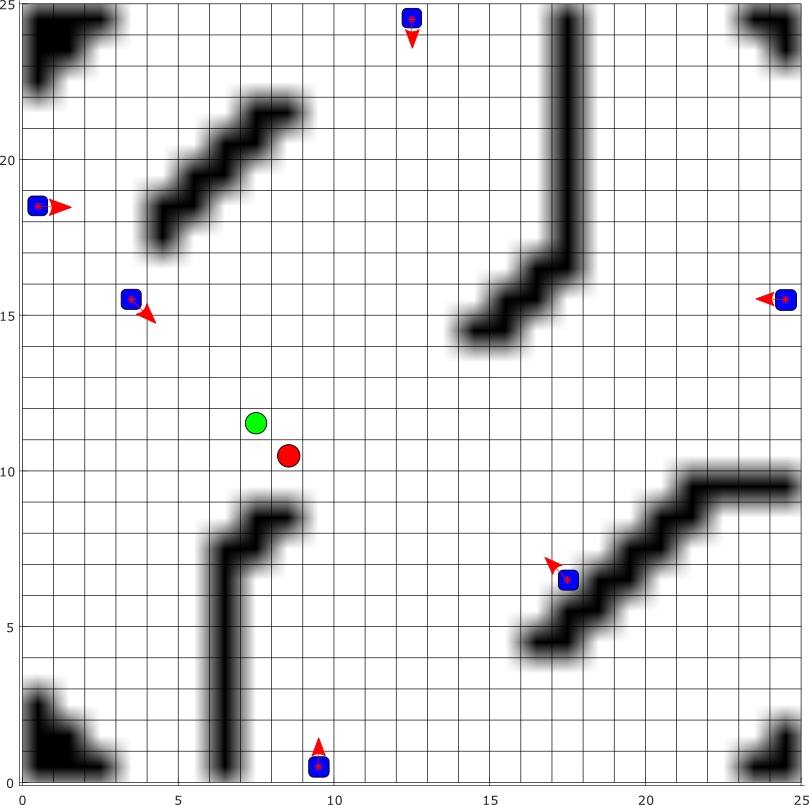
\includegraphics[width=.85\columnwidth]{./figs/exp1_corrected.pdf}}
	\caption{ The grid map of the environment, dark cells depict obstacles; 
	blue circles are trackers and the red circle is the ground truth location 
	of the maneuvering target; the green circle depicts the \axx{observation of 
	an agent.}}
	\label{fig:exp1}
\end{figure}

\section{Experiments} \label{sec:experiments}
The first experiment is concerned with a decentralized target pose estimation 
problem in a grid using multiple observers  connected through a changing  
topology network. Fig.~\ref{fig:exp1} depicts the 2D grid in which a target 
performs a random walk while six observers are trying to estimate its position. 
Each white cell is modeled as a single state of our HMM representing the 
position of the target on the grid. The observers' motion is deterministic; 
four of them are rooks moving along the borders and the other two are bishops 
moving diagonally on the grid. In order to detect the target, each observer 
emits a straight beam, normal to its direction of motion, as shown in the 
figure. The beam hits either the target or an obstacle. In the former case, the 
observer senses the position of the target 
based on a discrete one dimensional Gaussian distribution over the states that 
the beam has traversed; in the latter case, under the assumption of no false 
positives, the observer produces a `no target' symbol as an additional 
state (which is incorporated into the observation model by setting zero 
probabilities in 
the likelihood matrix for those states that beam has traveled through to hit 
a wall). 

\begin{figure}[t]
	\centering
	{\includegraphics[width=.85\columnwidth]{./figs/exp2.pdf}}
	\caption{Estimation performance in the tracking example}
	\label{fig:exp2}
\end{figure}

At each Markov transition, each observer carries out its decentralized 
estimation step for the position of the target, which is shared with other 
connected observers through a communication network. The network topology has 
two components; one has the rook observers and the other one has the bishops. 
The observers in each component are always connected while the link between the 
two components is intermittent. All communications occur at a higher rate than 
Markov transition steps, which allows the connected nodes to reach consensus 
over the shared information.

We evaluate the performance of the proposed Hybrid method during the phase 
where the rooks become disconnected from bishops, and are then reconnected 
after some interval. For purposes of comparison, each node performs three 
estimation processes. In one instance it uses our Hybrid method to fuse its 
prior along with the received priors. In the second instance it uses the ICF 
method to fuse its posterior along with the received posteriors. The third 
instance concerns a hypothetical god's-eye-view centralized estimator, to give 
a baseline for comparison. To quantify differences, we use the 
\axx{Bhattacharyya 
Coefficient \cite{bhattacharyya1946measure} between the estimation results and 
the 
centralized estimator. The Bhattacharyya coefficient can be used to evaluate 
the 
similarity of two probability mass functions, $\pi_1(\vect{X}), 
\pi_2(\vect{X})$ as:
\begin{equation}
\textstyle BC(\pi_1(\vect{X}),\pi_2(\vect{X})) = \sum_{\vect{x}\in 
\vect{X}}\sqrt{\pi_1(\vect{x}) \pi_2(\vect{x})}.
\end{equation}
In the case of $P_1= P_2$, complete similarity,  $BC(p_1,p_2)=1$, while 
$BC(p_1,p_2)=0$ means complete dissimilarity.}

Fig.~\ref{fig:exp2} compares the performance of the Hybrid and ICF methods, 
showing that the proposed method outperforms CF and is able to recover 
performance very close to centralized solution after reconnection.  Based on 
the Bhattacharyya coefficient, closeness between centralized and decentralized 
estimates drops during the interval of network partition. This is expected, 
since observers do not have access to all the information available to the 
centralized estimator. While the Hybrid method is able to start to recover 
immediately after reconnection, ICF continues with degraded performance even 
after reconnection owing to the fact that it ignores the correlations. 

Fig.~\ref{fig:exp2} also gives a detailed view of the performance of the Hybrid 
method and compares the estimation results of observer~3, a rook, and 
observer~5, a bishop, during three different time steps. The shaded area shows 
the time during which rooks are disconnected from the bishops. The higher 
difference between centralized and decentralized estimate for the fifth 
observer can be explained based on the fact that the bishop has less 
information at its disposal. However, after reconnection both groups are able 
to converge to the same value, which is very close to the centralized 
estimator. 

\begin{figure}[t]
	\centering
	{\includegraphics[width=0.98\columnwidth]{./figs/perf_measures_NGMD_GMD_curve6_corrected.pdf}}
	\caption{ Performance comparison between the proposed method and ICF. }
	\label{fig:gcf2}
\end{figure}

In a second experiment we have evaluated the robustness of the proposed method 
for networks with different likelihoods of link failure. We report the 
Bhattacharyya coefficient, and \axx{Hellinger} distance vs. link failure 
probability 
for a general decentralized HMM with a network of size 20 and state size 30 
with each node roughly connected to 10\% of the other nodes. We simulate the 
system multiple times, each time for 150 time steps but with different 
probability of link failure. At the beginning of each step, a 2 regular graph 
with 15 nodes is generated and, given a probability of failure for each link, 
some links in the graph will randomly be disconnected. The graph still remains 
connected some portion of the time, but this depends on the degree and 
probability of failure. If the regularity degree goes down or the probability 
of failure increases, more often than not, the graph becomes disconnected. In 
practice, for $p\geq0.05$, consensus methods that rely on \axx{full 
connectivity  
no longer succeed} since the network almost always suffers disconnection at 
some 
point in time.

We ran our method for 150 steps for a range of probabilities of link failure 
and compared performances with the ideal centralized result (which is obtained 
by assuming full connectivity at all times). The performance is evaluated by 
calculating the average value for the Bhattacharyya coefficient and determinant 
ratio measure at all steps and for all receptors.  Based on Fig. 
\ref{fig:gcf2}, for the case considered in this experiment, our decentralized 
estimator performs close to the ideal centralized one for $p\in[0.0 ,0.1]$, 
drastically outperforming ICF in all cases. This means that in the case 
considered here, our method can perform almost as well as the ideal estimator 
for an unreliable  network. Obviously the performance can vary from one system 
to another and under different network topologies, but the results show that 
the method can recover 
the performance of the centralized method despite operating on an unreliable 
network and, moreover, 
substantially outperforms ICF. This latter fact has also already been 
established 
theoretically.

%%%%%%%%%%%%%%%%%%%%%%%%%%%%%%%%%%%%%%%%%%%%%%%%%%%%%%%%%%%%%%%%%%%
\section{Conclusion} \label{sec:conclusion}
This paper proposes a distributed state estimator for discrete-state dynamic systems with non-Gaussian noise in networks with changing topology and those that do not remain connected all the time. Separating the process of consensus for the correlated and uncorrelated information was the key to achieving better performance compared to ICF alone. Evaluating the proposed method on a multi-agent tracking application and a high-dimensional HMM distributed state estimator problem showed substantial performance improvement compared to the state of the art. We are able to achieve robustness and recover performance after a disconnection interval occurs. 

%%%%%%%%%%%%%%%%%%%%%%%%%%%%%%%%%%%%%%%%%%%%%%%%%%%%%%%%%%%%%%%%%%%%%%%%%%%%%%%%
\bibliographystyle{IEEEtran} %\bibliographystyle{apalike}
\balance
\bibliography{RSS_2017}
%%%%%%%%%%%%%%%%%%%%%%%%%%%%%%%%%%%%%%%%%%%%%%%%%%%%%%%%%%%%%%%%%%%%%%%%%%%%%%%%

\end{document}
